\subsection{模的标量环的扩张}

设 A、B 为两个环，\(\rho: \mathbf{A} \to \mathbf{B}\) 为环同态；我们考虑由该同态定义的右A-模 \(\rho^{*}(B_{d})\)（§1，第13号）；这个A-模还具有左B-模结构，即 \(B_{s}\) 的结构，并且由于 \(b'(b\rho(a)) = (b'b)\rho(a)\)（对 \(a \in \mathbf{A}\) 及B中的 \(b\)、\(b'\)），B上的这两个模结构是相容的（§1，第14号）。这使我们可以对每个左A-模E，在张量积 \(\rho_{*}(B_{d}) \otimes_{\mathbf{A}} \mathbf{E}\) 上定义一个左B-模结构，使得 \(\beta'(\beta \otimes x) = (\beta'\beta) \otimes x\)（对B中的 \(\beta\)、\(\beta'\) 及 \(x \in \mathbf{E}\)）（§3，第3号）。这个左B-模称为借助 \(\rho\) 把标量环扩张到B而由E导出的模，记作 \(\rho^{*}(\mathbf{E})\) 或 \(\mathrm{E}_{(\mathbf{B})}\)（不致混淆时）。

对每个左A-模E，映射 \(\phi: x \mapsto 1 \otimes x\)（从E到A-模 \(\rho_*(\rho^*(\mathbf{E}))\)）是A-线性的，且集合 \(\phi(\mathbf{E})\) 生成B-模 \(\rho^*(\mathbf{E})\)。进而，对每个左B-模F与每个A-线性映射 \(f\)（从E到A-模 \(\rho_*(\mathbf{F})\)），存在唯一的B-线性映射 \(\tilde{f}\)（从 \(\rho^*(\mathbf{E})\) 到F），使得 \(\tilde{f}(1 \otimes x) = f(x)\)（对所有 \(x \in \mathbf{E}\)）。

B 可借助 \(\rho\) 视为一个 (B, A)-双模；于是存在一个典范的 Z-模同构

\[
\operatorname{Hom} _ {\mathbf {B}} (\mathbf {B} \otimes_ {\mathbf {A}} \mathbf {E}, \mathbf {F}) \rightarrow \operatorname{Hom} _ {\mathbf {A}} (\mathbf {E}, \operatorname{Hom} _ {\mathbf {B}} (\mathbf {B} _ {s}, \mathbf {F}))\tag{1}
\]

这正如§4第1号命题1所示。但左A-模 \(\mathrm{Hom}_{\mathbf{B}}(\mathbf{B}_{s},\mathbf{F})\) 典范地等同于 \(\rho^{*}(\mathbf{F})\)：因为按定义（§1，第14号），对元素 \(y\in \mathbf{F}\) 对应着同态 \(\theta (y)\colon \mathbf{B}_s\to \mathbf{F}\)，它满足 \((\theta (y))(1) = y\)；于是对所有 \(\lambda \in \mathbf{A}\)，对 \(\rho (\lambda)y\in \mathbf{F}\) 对应着同态 \(\mu \mapsto \mu \rho (\lambda)y\)（从 \(\mathbf{B}_s\) 到 \(\mathbf{F}\) 的），它正是 \(\lambda \theta (y)\)（对 \(\mathrm{Hom}_{\mathbf{B}}(\mathbf{B}_{s},\mathbf{F})\) 的左A-模结构而言）（§1，第14号）。利用这一等同，我们因此得到一个典范Z-模同构，即 (1) 的逆

\[
\delta : \operatorname{Hom} _ {\mathbf {A}} (\mathbf {E}, \rho_ {*} (\mathbf {F})) \rightarrow \operatorname{Hom} _ {\mathbf {B}} (\rho^ {*} (\mathbf {E}), \mathbf {F})\tag{2}
\]

并且由定义立即得出，若 \(\delta(f) = \bar{f}\)，则 \(\bar{f}(1 \otimes x) = f(x)\)（对所有 \(x \in \mathbf{E}\)）。特别地，映射 \(\phi_{\mathbb{E}}: x \mapsto 1 \otimes x\) 恰好就是

\[
\phi_ {\mathbf {E}} = \delta^ {- 1} (1 _ {\rho^ {*} (\mathbf {E})}).\tag{3}
\]

因此，命题1得证。该映射 \(\phi_{\mathbf{E}}: \mathbf{E} \to \rho_{*}(\rho^{*}(\mathbf{E}))\) 被称为典范的。

注. (1) 命题1表明，由 \(\mathbf{E}_{(\mathbf{B})}\) 与 \(\phi_{\mathbb{E}}\) 组成的有序对是泛映射问题（集合论，IV，§3，第1号）的一个解，其中 \(\Sigma\) 是左B-模结构的物种（态射为B-线性映射），而 \(\alpha\)-映射是E到某个B-模中的A-线性映射。

\begin{enumerate}
\def\labelenumi{(\arabic{enumi})}
\setcounter{enumi}{1}
\item
  若E是一个 \((\mathbf{A}, (\mathbf{C}_{i}^{\prime}); (\mathbf{D}_{j}^{\prime}))\) -多模且F是一个 \((\mathbf{B}, (\mathbf{C}_{h}^{\prime\prime}); (\mathbf{D}_{k}^{\prime\prime}))\) -多模，则同构(2)关于两边的 \(((\mathbf{D}_{j}^{\prime}), (\mathbf{C}_{h}^{\prime\prime}); (\mathbf{C}_{i}^{\prime}), (\mathbf{D}_{k}^{\prime\prime}))\) -多模结构是线性的（§1，第14号及§3，第4号）。
\item
  设E为左A-模，a为A的双边理想，且 \(\rho:A\to A/a\) 为典范同态。在§3第6号命题6推论2的记号下，A-模E/aE被a零化，因此典范地具有左(A/a)-模结构（§1，第12号）；显然，§3第6号命题6推论2中定义的典范映射 \(\pi:\rho^{*}(E)\to E/aE\) 对于(A/a)-模结构是同构。
\end{enumerate}

推论。设E，E'为两个左A-模；对每个A-线性映射u: E → E'，v = l\_B ⊗ u是使下图交换的唯一B-线性映射

\pandocbounded{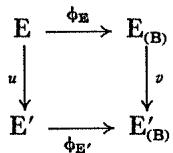
\includegraphics[keepaspectratio]{images/part002_74d11806.jpg}}

（其中 \(\phi_{\mathbf{E}}\) 与 \(\phi_{\mathbf{E}'}\) 是典范映射）。

只需将命题1应用于A-同态 \(\phi_{\mathbf{E}'} \circ u: \mathbf{E} \to \mathbf{E}_{(\mathbf{B})}'\)。

上述推论中定义的映射 \(v\) 记作 \(\rho^{*}(u)\) 或 \(u_{(B)}\)。若 \(E''\) 是第三个左A-模且 \(v: E' \to E''\) 为A-线性映射，则显然

\[
\left(v \circ u\right) _ {(\mathbf {B})} = v _ {(\mathbf {B})} \circ u _ {(\mathbf {B})}.
\]

模的算子环的扩张是一种可传递的运算；确切地说：

命题2. 设 \(\rho: \mathbf{A} \to \mathbf{B}\) , \(\sigma: \mathbf{B} \to \mathbf{C}\) 是环同态。对每个左A-模E，存在唯一的C-同态

\[
\sigma^ {*} (\rho^ {*} (\mathrm{E})) \rightarrow (\sigma \circ \rho) ^ {*} (\mathrm{E})\tag{4}
\]

它把 \(1 \otimes (1 \otimes x)\) 映为 \(1 \otimes x\)（对所有 \(x \in E\)），且该同态是双射。

\(\sigma^{*}(\rho^{*}(\mathbf{E}))\) 与 \((\sigma \circ \rho)^{*}(\mathbf{E})\) 的底层Z-模分别是 \(\mathbf{C} \otimes_{\mathbf{B}} (\mathbf{B} \otimes_{\mathbf{A}} \mathbf{E})\) 与 \(\mathbf{C} \otimes_{\mathbf{A}} \mathbf{E}\)。存在一个典范Z-同构 \(\mathbf{C} \otimes_{\mathbf{B}} (\mathbf{B} \otimes_{\mathbf{A}} \mathbf{E}) \to (\mathbf{C} \otimes_{\mathbf{B}} \mathbf{B}) \otimes_{\mathbf{A}} \mathbf{E}\) （§ 3，第8号，命题8），它对于两侧的左C-模结构也是C-同构。此外，C-模C ⊗B B在映射γ ⊗ β到γσ(β)的同构下典范地等同于C-模Cs（§ 3，第4号，命题4），并且该同构也是对于由ρ定义的C ⊗B B上的右A-模结构和由σ ∘ ρ定义的C上的右A-模结构的同构。因此，存在一个典范同构

\[
(\mathbf {C} \otimes_ {\mathbf {B}} \mathbf {B}) \otimes_ {\mathbf {A}} \mathbf {E} \rightarrow \mathbf {C} \otimes_ {\mathbf {A}} \mathbf {E}
\]

于是就得到；将它与同构

\[
\mathbf {C} \otimes_ {\mathbf {B}} (\mathbf {B} \otimes_ {\mathbf {A}} \mathbf {E}) \rightarrow (\mathbf {C} \otimes_ {\mathbf {B}} \mathbf {B}) \otimes_ {\mathbf {A}} \mathbf {E}
\]

复合，就得到所需的典范同构。

若 \(\phi, \phi'\) 和 \(\phi''\) 分别记典范映射 \(E \to \rho^*(E)\) , \(\rho^*(E \to) \sigma^*(\rho^*(E))\) 和 \(E \to (\sigma \circ \rho)^*(E)\) ,则在命题2的典范同构下，\(\phi' \circ \phi\) 与 \(\phi''\) 等同。

命题3. 设A，B为两个交换环， \(\rho: \mathbf{A} \to \mathbf{B}\) 为环同态，且 E、E' 是两个 A-模。存在唯一的 B-同态

\[
\mathbf {E} _ {(\mathbf {B})} \otimes_ {\mathbf {B}} \mathbf {E} _ {(\mathbf {B})} ^ {\prime} \rightarrow (\mathbf {E} \otimes_ {\mathbf {A}} \mathbf {E} ^ {\prime}) _ {(\mathbf {B})}\tag{5}
\]

它把 \((1 \otimes x) \otimes (1 \otimes x')\) 映为 \(1 \otimes (x \otimes x')\)（对 \(x \in \mathbf{E}\)、\(x' \in \mathbf{E}'\)），且该同态是双射。

（5）的左边可写成 \((\mathbf{B} \otimes_{\mathbf{A}} \mathbf{E}) \otimes_{\mathbf{B}} (\mathbf{B} \otimes_{\mathbf{A}} \mathbf{E}')\)，且（因A与B交换）与 \((\mathbf{E} \otimes_{\mathbf{A}} \mathbf{B}) \otimes_{\mathbf{B}} (\mathbf{B} \otimes_{\mathbf{A}} \mathbf{E}')\) 等同；后一个乘积依次等同于 \(\mathbf{E} \otimes_{\mathbf{A}} (\mathbf{B} \otimes_{\mathbf{B}} \mathbf{B}) \otimes_{\mathbf{A}} \mathbf{E}'\) , \(\mathbf{E} \otimes_{\mathbf{A}} (\mathbf{B} \otimes_{\mathbf{A}} \mathbf{E}')\) , \(\mathbf{E} \otimes_{\mathbf{A}} (\mathbf{E}' \otimes_{\mathbf{A}} \mathbf{B})\) ，最终等同于 \((\mathbf{E} \otimes_{\mathbf{A}} \mathbf{E}') \otimes_{\mathbf{A}} \mathbf{B}\) ，这利用了张量积的结合性（§3，第8号，命题8）、§3第4号命题4以及A与B的交换性。所需的同构是这些相继的典范同构的复合。

显然，若S是E的一个生成系，则S在典范映射 \(E \rightarrow E_{(B)}\) 下的像是 \(E_{(B)}\) 的一个生成系；特别地，若E是有限生成的A-模，则 \(E_{(B)}\) 是有限生成的B-模。

命题4. 设E是具有基 \((a_{\lambda})_{\lambda \in L}\) 的A-模；若 \(\phi : x \mapsto 1 \otimes x\) 是E到 \(\rho^{*}(\mathbf{E})\) 的典范映射，则 \((\phi(a_{\lambda}))_{\lambda \in L}\) 是 \(\rho^{*}(\mathbf{E})\) 的一组基。若 \(\rho\) 是单射，则 \(\phi\) 亦然。

第一个断言直接由§3第7号命题7的推论1得出。此外，对A中元素的每个有限支撑族 \((\xi_{\lambda})_{\lambda \in L}\)，有 \(\phi\left(\sum_{\lambda \in L} \xi_{\lambda} a_{\lambda}\right) = \sum_{\lambda \in L} \rho(\xi_{\lambda}) \phi(a_{\lambda})\)，因而关系 \(\phi\left(\sum_{\lambda \in L} \xi_{\lambda} a_{\lambda}\right) = 0\) 等价于 \(\rho(\xi_{\lambda}) = 0\)（对所有 \(\lambda \in L\)），由此得出第二个断言。

推论. 对每个投射A-模E，B-模 \(\rho^{*}(\mathbf{E})\) 是投射的。若进一步 \(\rho\) 是单射，则E到 \(\rho^{*}(\mathbf{E})\) 的典范映射是单射。

由假设，存在一个包含E的自由A-模M，且E在M中有一个补子模F。由§3第7号命题7直接可得，\(\mathbf{M}_{(\mathbf{B})}\) 等同于 \(\mathbf{E}_{(\mathbf{B})}\) 与 \(\mathbf{F}_{(\mathbf{B})}\) 的直和，且若 \(\phi\) 和 \(\psi\) 是典范映射 \(\mathbf{E} \to \mathbf{E}_{(\mathbf{B})}\) 和 \(\mathbf{F} \to \mathbf{F}_{(\mathbf{B})}\)，则典范映射 \(\mathbf{M} \to \mathbf{M}_{(\mathbf{B})}\) 就是 \(x + y \mapsto \phi(x) + \psi(y)\)。该推论由命题4应用于A-模M直接得出。

当E是右A-模时，我们类似地记 \(\rho^{*}(\mathbf{E}) = \mathbf{E} \otimes_{\mathbf{A}} \rho_{*}(\mathbf{B}_{s})\)，此时将 B 视为 (A, B)-双模，且 \(\rho^{*}(\mathbf{E})\) 上的右B-模结构满足 \((x \otimes \beta)\beta' = x \otimes (\beta\beta')\)（对 \(\beta \in B, \beta' \in B\) 和 \(x \in E\)）。我们把本小节及下一小节中相应于右模的结果的陈述留给读者自行完成。

注记（4）. 考虑左A-模 \(\rho_{*}(B_{s})\)（由 \(\rho\) 定义），并且对每个左A-模E，考虑Z-模

\[
\tilde {\rho} (\mathbf {E}) = \operatorname{Hom} _ {\mathbf {A}} \left(\rho_ {*} \left(\mathbf {B} _ {s}\right), \mathbf {E}\right).\tag{6}
\]

由于 \(\rho_{*}(\mathbf{B}_{s})\) 具有右B-模结构，在 \(\tilde{\rho}(\mathbf{E})\) 上导出一个左B-模结构（\(\S 1\)，第14号），使得若 \(u \in \tilde{\rho}(\mathbf{E})\) 且 \(b' \in \mathbf{B}\)，则 \(b'u\) 是同态 \(b \mapsto u(bb')\)（从 \(\rho_{*}(\mathbf{B}_{s})\) 到 \(\mathbf{E}\)）。我们进一步定义一个称为典范的A-线性映射

\[
\eta : \rho_ {*} (\tilde {\rho} (\mathbf {E})) \rightarrow \mathbf {E}\tag{7}
\]

它把每个同态 \(u \in \tilde{\rho}(\mathbf{E})\) 对应到元素 \(u(1)\)（在 \(\mathbf{E}\) 中）。由于 \(\mathbf{B}\) 可借助 \(\rho\) 被视为一个(A, B)-双模，对每个左B-模 \(\mathbf{F}\)，存在一个典范的 \(\mathbf{Z}\)-模同构

\[
\operatorname{Hom} _ {\mathbf {A}} \left(\rho_ {*} (\mathrm{B} _ {s}) \otimes_ {\mathrm{B}} \mathrm{F}, \mathrm{E}\right)\rightarrow \operatorname{Hom} _ {\mathbf {B}} (\mathrm{F}, \operatorname{Hom} _ {\mathbf {A}} \left(\rho_ {*} (\mathrm{B} _ {s}), \mathrm{E}\right))
\]

（§1，第1号，命题1）。由于左A-模 \(\rho^{*}(B_{s}) \otimes_{B} F\) 依据§3第4号命题4典范地等同于 \(\rho_{*}(F)\)，我们得到一个典范Z-模同构，即上述同构的逆

\[
\operatorname{Hom} _ {\mathbf {B}} (\mathbf {F}, \tilde {\rho} (\mathbf {E})) \rightarrow \operatorname{Hom} _ {\mathbf {A}} (\rho_ {*} (\mathbf {F}), \mathbf {E})\tag{8}
\]

它把每个从F到 \(\tilde{\rho}(\mathbf{E})\) 的B-线性映射g对应到复合映射 \(\eta \circ g\)，视为从 \(\rho_{*}(\mathbf{F})\) 到E的A-线性映射。特别地，在命题2的假设下，若把F换成 \(\sigma_{*}(\mathbf{C}_{s})\)，则得到典范C-同构

\[
\tilde {\sigma} (\tilde {\rho} (\mathbf {E})) \rightarrow (\sigma \circ \rho) ^ {\sim} (\mathbf {E}).\tag{9}
\]

